\documentclass[11pt,a4paper]{article}
\usepackage[utf8]{inputenc}
\usepackage{amsmath}
\usepackage{amsfonts}
\usepackage{amssymb}
\usepackage{graphicx}
\usepackage{multirow}
%\usepackage[margin=1.5 cm]{geometry}
\usepackage[table]{xcolor}
\usepackage{hyperref}
\graphicspath{ {./images/} }
\author{Bianca}
\DeclareMathOperator*{\argmin}{argmin}
\DeclareMathOperator*{\argmax}{argmax}
\DeclareMathOperator*{\diag}{diag}
\DeclareMathOperator*{\sign}{sign}
\DeclareMathOperator*{\x}{\textbf{x}}
\begin{document}
\begin{flushleft}
\section{Begriffe}
\begin{table}[]
{\rowcolors{1}{black!10!}{black!5}
\begin{tabular}{l p{0.2\textwidth} l p{0.2\textwidth} l p{0.2\textwidth}}
$O$ & is a set of objects  & Mushrooms \\
$C$ & is a set of classes  & essbar oder nicht \\
$X$ & Set/ Menge der Feature Vektoren & Vektoren mit den Eigenschaften der Pilze                 \\
\textbf{X}                                                             & Feature Vektor; Feature Space; Feature Domain                                      &                                                                                                                       \\
\textbf{x}                                                             & one feature vector                                                                 & ein Pilz                                                                                                              \\
x                                                                      & single feature                                                                     & ein eigenschaft von einem Pilz (z.B. braun)                                                                          \\
\textbf{w}                                                             & Weight-Vektor                                                                      &                                                                                                                       \\
$D={(x_1, c(x_1)),…, ((x_n, c(x_n))}$                         & classification knowledge alias the example set                                     & schon bestimmte Pilze                                                                                                 \\
\textit{D = \{(x1, y1), … , ((xn, yn)\}}                               & same but for regression                                                            & Mietpreise von Wohnungen                                                                                             \\
$\alpha(o) = x$                                                               & model formation function                                                           & Funktion zur Bestimmung der Pilz-Eigenschaften                                                                       \\
y(x) (Ziel y(x) = c(x))                                                & model function/ classifier                                                         & Bestimmung ob essbar anhand der Eigenschaften                                                                          \\
\textit{$\gamma(o)$ mit $O \rightarrow C$}                                                & ideal target function / ideal classifier für O                                     & Pilzexperte der Pilze bestimmt                                                                                         \\
c(x) mit c: $X \rightarrow C$                                                      & ideal target function/ ideal classifier for X ; indirekt gegeben durch D           & Theoretische Ideale Bestimmung aller Pilze                                                                            \\
$h(x), h: X \rightarrow \{0,1\}$                                                   & hypothesis/ model function  to approximate c(x)                                    & wenn es sonnig ist mache ich Sport (Regeln/ Hypothesen  zur classification)                                            \\
$y_i$                                                                     & ground truth for $xi \in X $                                                            & der Mietpreis für eine Wohnung                                                                                       \\
\textit{H}                                                             & hypothesis space                                                                   & Menge alle möglichen Hypothesen/Regeln                                                                                 \\
$V_{H,D} = \{h(x) | h(x) \in  H \wedge $ & \multirow{2}{0.2\textwidth}{version space : Menge aller möglichen Regeln (h(x)) die sich aus D ableiten lassen} & \multirow{2}{0.2\textwidth} {Wenn es sonnig ist gehe ich raus, Wenn es warm ist gehe ich raus, wenn es windig ist und scheint gehe ich raus, etc.}  \\
$( \forall(x, c(x)) \in D : h(x) = c(x)) \}$ & &  \\
$ \mathcal{X} \in X / \mathcal{C} \in C$ & random variables & ein random Pilz bzw. eine random Klasse                                       \\
$p(x, c) = P(X=x, C=c)$                                                  & the probability of the joint event that $x \in X$ \& x belongs to class $c \in C   $ & die Wahrscheinlichkeit das ein Pilz zu einer bestimmten Klasse gehört                                                  \\
$\eta$                                                                      & {learning rate}                                                                & a small positiv constant                                                                                              \\
                                                                       & p- dimensional direction vector $w \rightarrow = (w1, . . . , wp) T$ &                                                                                                                       \\
                                                                       & p + 1)-dimensional hypothesis $w = (w0, w1, . . . , wp) T$                                                                                                                                             & 
\end{tabular}
}
\end{table}
\section{Definition Formel \& Algorithmen}

\subsection{Specification of learning tasks}
    \textbf{Realworld $\rightarrow$ Modelworld} \newline
    \begin{enumerate}
    \item \textbf{Reale Welt:}
    \end{enumerate}
    \begin{itemize}
        \item $O$ - Menge an Objekten
        \item $C$ - Menge an Klassen
        \item $\gamma: O \rightarrow C$ - idealer Classifier für $O$
    \end{itemize}
    \quad Aufgabe-Klassifizierung:
    \begin{itemize}
        \item bestimme von $o \in O$ die Klasse $\gamma(o) \in C$
    \end{itemize}
    
    \begin{enumerate}
        \setcounter{enumi}{1}
        \item \textbf{Model Welt}
    \end{enumerate}
     \begin{itemize}
         \item $X$ - Menge von feature Vektoren
         \item $C$ - Menge von Klassen
         \item $c: X \rightarrow C$ - idealer Classifier für $X$ \textit{(c ist unbekannt)}
         \item $ D =$ \{($\textbf{x}_1,c(\textbf{x}_1)),\ \dots\ ,(\textbf{x}_n, c( \textbf{x}_n)) $\} - Menge von Beispielen \textit{(bereits klassifiziert)}
     \end{itemize}
    Todo: Schätze $c(\mathbf{x})$, welche implizit durch $D$ gegeben sind, durch
    \newline \quad Model-Funktion $y(\mathbf{x})$ 
    \newline\newline
\subsection{Machine Learning:}
    \begin{enumerate}
    	\item Collect real-world examples of the form $(o, \gamma (o) ), o \in O $
    	\item abstract the objects towards feature vectors $ \textbf{x} \in X$, where $\textbf{x} = \alpha (0)$
        \item Formuliere Model-Function: $y: X \rightarrow C, \mathbf{x} \mapsto y(\mathbf{x})$
        \item Nutze Statistik, Theorie und Algorithmen aus ML um den fit zwischen $c(\mathbf{x})$ und $y(\mathbf{x})$ zu Maximieren, sodass $y(\textbf{x} ) \approx c( \textbf{x} ) \approx \gamma (o)$
    \end{enumerate}
    \includegraphics[width= 0.8\textwidth]{modelworld}
    
    \subsection{LMS: Least Mean Squared}
    Ziel: Fitting $y(x)$; Anpassung der weights, sodass Klassifizierungsfehler möglichst gering sind. \\~\\
    Input: $D$ - Trainingsdaten ($\mathbf{x},c(\mathbf{x})$) mit \textbf{x}$\in \textbf{R}^p$ und Zielklasse c(\textbf{x}) 
    $\eta$ Learning rate, kleine positive Konstante
    \\~\\
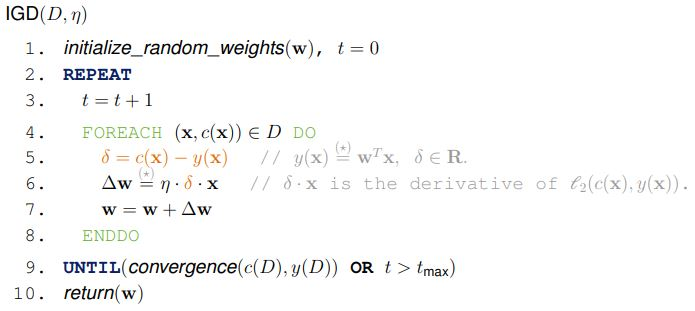
\includegraphics[width=\textwidth]{IGD}

\subsection{Lineare Regression}

Grundformel für lineare Gerade, mit: \newline
$y(x)$ - abhängige Variabel
$x$ - unabhängige Variable
$w_1$ - Anstieg der Geraden
$w_0$ - Schnittpunkt der y-Achse
\begin{equation}
    y(x)=w_o+w_1\cdot x
\end{equation}
Wobei das minimale $w_0$ und $w_1$ sich ergeben aus:
\begin{equation}
    w_1=\frac{\sum\limits^{n}_{i=1}(x_i-\overline{x}\cdot(y_i-\overline{y})}{\sum\limits_{i=1}^{n}(x_i-\overline{x}^2}
\end{equation}
\begin{equation}
    w_0=\overline{y}-w_1\cdot\overline{x}
\end{equation}

\paragraph{Goodness of Modelfit, Regressionserror}
Residual sum of Squares(RSS). \newline
Der Residue wird aus der Differenz zwischen (beobachteten) Realwelt-Wert $y_i$ und geschätzten/modelierten Wert $y(\mathbf{x}_i)$
\begin{equation}
    RSS(\mathbf{w}) = \sum^{n}_{i=1}(y_i-y(\mathbf{x}_i))^2
\end{equation}

\paragraph{Higher-Dimensional Feature Space} ML:ll-16


\subsection{Concept Learning}
Setting:\newline
$X$ - Menge an Feature Vektoren\newline
$C$ - Ist eine Menge mit zwei Klassen \textit{Beipiel: \{0,1\},\{ja, nein\}} \newline
$c: X \rightarrow C$ -idealer Klssifizierer für $X$ \newline
$D=\{(\mathbf{x}_1,´c(\mathbf{x}_1)),\dots,(\mathbf{x}_n,c(\mathbf{x}_n))\} \subseteq X \times C$ - Menge mit Beispielen \newline
Todo: \newline
Schätze $c(x)$, was implizit durch $D$ mit feature-Value-Muster


\newpage
\section{Definitionen Text}
\subsection{Supervised learning} 
    Eine Funktion mithilfe von input-output-Daten lernen; \newline
    automatisierte Klassifikation mit von Menschen bereits klassifizierten Daten als Grundlage \newline
    \textit{Beispiel: optical character recognizition}
    
\subsection{Unsupervised learning}
    identifiziert/findet selbstständig Muster und Strukturen in Daten; \newline
    \begin{itemize}
        \item automatisierte Kategorisierung durch Cluster Analysis
        \item Parameter Optimierung durch Expectation Maximation
        \item Feature Extrahierung durch Factor Analysis
    \end{itemize}
    \textit{Beispiel: intrusion detection in a network data stream}
    
\subsection{Reinforcement learning}
    "Learn, adapt, or optimize a behavior strategy in order to maximize the ownbenefit by interpreting feedback that is provided by the environment."
    \textit{Beispiel: program to play tetris}

\subsection{Feature Vektor}
    Ein Feature Vektor ist ein Vektor in dem jede Dimension eine Eigenschaft(Feature) des beschriebenen Objektes enthält.\newline
    \textbf{x} =
    $\begin{bmatrix}
    x_1\\
    x_2\\
    .\\
    .\\
    .\\
    x_n
    \end{bmatrix}$
    \quad Besipiel: \textbf{Gitarre} = 
    $\begin{bmatrix}
    Farbe: blau\\
    Baujahr: 1997\\
    Material: Holz\\
    Elektrisch: ja\\
    \end{bmatrix}$


\subsection{Ground Truth}
Überprüfung der Klassifizierung eines Lernprozesses auf Richtigkeit für gewolltes Model.\newline
\textit{Beispiel: Überprüfung eines Spamfilter nach falsch kategorisierten Mails}

\section{Linear Models}
\subsection{Overfitting}
\begin{itemize}
\item fitting: der Prozess die Parameter einer Modelfunktion y so anzupassen das sie der der Beispieldaten D am besten passen
\item overfiiting: "Fitting the data more than is warranted"
\item alias besser passen als berechtigt?
\item Gründe:
	\begin{itemize}
	\item zu komplizierte Modefunktion (zu viele Features) 
	\item zu wenig Daten in D
	\item zu viel Datenrauschen
	\item D ist zu biased alias nicht repräsentativ 
	\end{itemize}
\item Folgen:
	\begin{itemize}
	\item kleiner Error auf $D_{tr}$ anber großer Error auf $D_{test}$ und IRL
	\item loss of inductive Bias
	\item increase of variance as a result of sensitivity to noise
	\end{itemize}
\item Overfitting finden: 
	\begin{itemize}
	\item Visuell untersuchen für Fälle mit Dimensionen $<3$ sonst embedding oder 		projizieren  in kleinere Dimensionen
	\item Validieren: wenn $Err_{fit} = Err_{val}(y) - Err_{tr}(y)$ zu groß ist
	\end{itemize}
\item Overfitting vermeiden:
	\begin{itemize}
	\item Early stopping through model selection: nach m schritten überprüfen ob sich $ Err_{fit}$ noch verkleinert und stoppen wenn er sich vergrößert
	\item Qualität (schlechte Beispiele raus) und / oder Quantität (mehr Daten gleichen Rauschen aus) von D verbessern
	\item Manually enforcing a higher bias by using a less complex hypothesis space alias Removing Features: In this approach, irrelevant features are removed from the dataset.
This enhances the algorithm’s ability to generalize
	\item Regularization (WUHU!)
	\end{itemize}
\end{itemize}
\subsubsection{Well- and Ill-posed problems}
A mathematical problem is called well-posed if
\begin{itemize}
\item[1.] a solution exists,
\item[2.] the solution is unique,
\item[3.]the solution’s behavior changes continuously with the initial conditions.
\end{itemize}
Otherwise, the problem is called ill-posed.

\subsection{Regularization}
Automatic adjustment of the loss function to penalize model complexity. \\
Let $L(\textbf{w}$ denote a loss function used to optimize the parameters \textbf{w} of a model
function $y(\textbf{x})$. Regularization introduces a trade-off between model complexity and inductive bias:

$$\mathcal{L}(\textbf{w}) = L(\textbf{w}) + \lambda * R(\textbf{w})$$

where $\lambda \geq 0$ controls the impact of the regularization term $R(\textbf{w}) \geq 0$. $\mathcal{L} $ is called “objective function”.

\subsubsection{Regularized Linear Regression}

$$\mathcal{L}(\textbf{w}) = \displaystyle\sum_{i=1}^{n}(y_i - \textbf{w}^T \textbf{x}_i)^2 + \lambda \cdot \overrightarrow{w}^T \overrightarrow{w}$$
Estimate \textbf{w} by minimizing the residual sum of squares:
$$\hat{w}= \argmin_{\mathbf{w\in R^{p+1}}} \mathcal{L}(\textbf{w}) $$

$$ \leadsto RSS(\textbf{w}) = (\textbf{y} -\textbf{Xw})^T (\textbf{y} -\textbf{Xw})+ \lambda \textbf{w}^T \textbf{w} $$

Ableitung bilden um RSS(\textbf{w}) zu minimieren und man kommt auf:

$$ \textbf{w} = (X^T X + \diag(0,\lambda, ..., \lambda))^{-1} X^T \textbf{y} $$

$$ \diag(0,\lambda, ..., \lambda) = \begin{bmatrix}
       0 & 0 & 0 & ... & 0 \\[0.3em]
       0 & \lambda & 0 & ... & 0 \\[0.3em]
       0 & 0 & \lambda & ... & 0 \\[0.3em]
       \vdots & \vdots & \vdots & \ddots & \vdots\\[0.3em]
       0 & 0 & 0 & ...& \lambda
     \end{bmatrix} $$
     
$$ \hat{y}(\textbf{x}_i) = \mathbf{\hat{w}}^T \textbf{x}_i $$

Um so höher $\lambda$ um so einfacher ist die Funktion - Regularization archived!

\section{Neural Networks}

\subsection{Perception Learning}
Idee: Lass mal ein Gehirn programmieren! \\
Typisches Beispiel: Schrifterkennung 

$$ y(\textbf{x}) = 1 \Leftrightarrow (\displaystyle\sum_{j=0}^p w_j x_j  ) \geq 0  $$

sonst ist y(\textbf{x}) = 0

\begin{itemize}
\item wenn $w_0 = -\theta$ und $x_0 = 1$(canonical form) 
\item sonst $ y(\textbf{x}) = 1 \Leftrightarrow (\displaystyle\sum_{j=1}^p w_j x_j - \theta ) \geq 0 $
\item $ 0 = w_0 + w_1 * x_1 + w_2 * x_2 $ für 2D Fälle
\end{itemize}

\subsubsection{PT Algorithm}
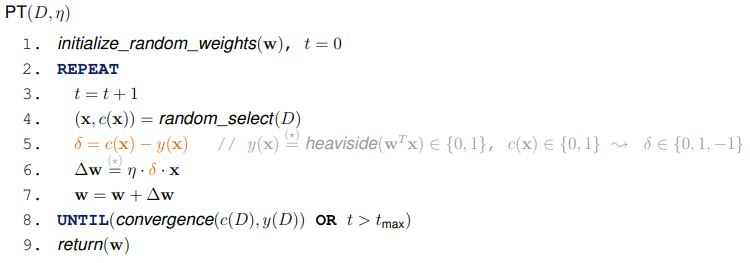
\includegraphics[width=\textwidth]{PT}
\begin{itemize}
\item If a separating hyperplane between $X_0$ and $X_1$ exists, the PT algorithm will
converge. If no such hyperplane exists, convergence cannot be guaranteed.
\item A separating hyperplane can be found in polynomial time with linear
programming. The PT Algorithm, however, may require an exponential
number of iterations.
\item Classification problems with noise are problematic
\end{itemize}
\subsection{Gradient Descent}
\begin{itemize}
\item Finde den kürzesten Weg in ein Min/Max über partielle Ableitungen
\item The gradient of a function is the direction of steepest ascent or descent.
\item in der VL ist ein Beweis den ich nicht abtippe weil irrelevant 
\end{itemize}
\subsubsection{Linear Regression + Squared Loss}

$$ L_2(\textbf{w}) = \dfrac{1}{2} \cdot \displaystyle\sum_{(\textbf{x}, c(\textbf{x})) \in D} (c(\textbf{x}) - y(\textbf{x}))^2$$

Jetzt müssen wir für jedes $w_i$ aus \textbf{w} eine partielle Ableitung machen um den weight vector zu updaten ($ \textbf{w} = \textbf{w} + \Delta \textbf{w}$)

$$ \Delta\textbf{w} =  \dfrac{ \delta }{\delta w_i} L_2 (\textbf{w}) = \eta \cdot \displaystyle\sum_D (c(\textbf{x}) - \textbf{w}^T\textbf{x}) \cdot \textbf{x}$$

$\eta$ = learning rate - a small positiv constant - legen wir selbst fest

\subsubsection{The Batch Gradient Descent (BGD) Algorithm}
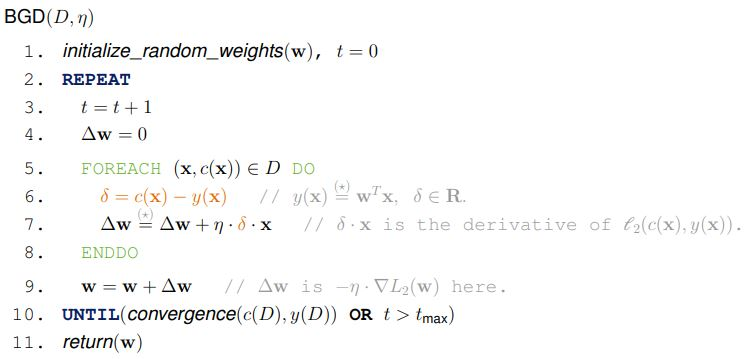
\includegraphics[width=\textwidth]{BGD}
\begin{itemize}
\item wichtig: immer wenn irgendwo $\textbf{w}^T\textbf{x}$ steht haben wir $x_0 = 1$ zu \textbf{x} hinzugefügt
\item funktionsweise BGD. wir berechnen über die Ableitung in welche Richtung wir müssen und gehen dann einen Schritt der große $\eta$
\item die "convergence" schaut ob der Squared Loss noch größer als ein $\varepsilon$ ist (das wir auch festlegen)
\item BGD ist nicht der schnellste (bestenfalls linear) aber sehr einfach (Newton-Raphson algorithm, BFGS algorithm sind z.B. schneller)
\item BGD nimmt den global loss: loss of all examples in D (“batch gradient descent”)(Schritt in Richtung die für alle Punkte am besten ist)
\item man kann auch den (squared) loss in Bezug auf einzelne Beispiele nehmen (pointwise loss) (dann gehts halt im Zickzack runter)
\ berechnet sich dann $\ell_2(c(\textbf{x}), y(\textbf{x})) = \dfrac{1}{2} (c(\textbf{x})- \textbf{w}^T\textbf{x})^2$
\item bzw. die weight adaptation: $ \Delta\textbf{w} = \eta \cdot (c(\textbf{x}) - \textbf{w}^T \textbf{x}) \cdot \textbf{x} $
\item für $BGD_\sigma$ wird Zeile 9 zu  \\ $\textbf{w} = \textbf{w} + \Delta \textbf{w} + \eta \cdot 2 \lambda \cdot \binom{0}{\overrightarrow{\textbf{w}}}$
\end{itemize}
\subsubsection{The Incremental Gradient Descent IGD Algorithm}
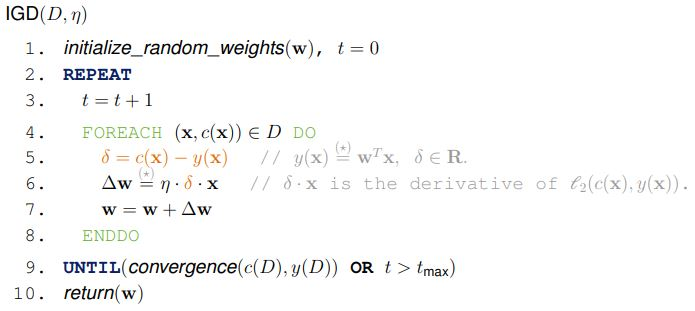
\includegraphics[width=\textwidth]{IGD}
\begin{itemize}
\item kleinere Schritte als BGD
\item  can better avoid getting stuck in a local minimum of the loss function then BGD
\end{itemize}
\subsubsection{Linear Regression + Squared Loss}
$$ L_{0/1}(\textbf{w}) = \displaystyle\sum_D \dfrac{1}{2} \cdot (c(\textbf{x})  - \sign (\textbf{w}^T \textbf{x} )) $$

$L_{0/1}8\textbf{w})$ cannot be expressed as a diffrentiable function alias es kann nicht abgeleitet werden damit ist gradient descent nicht möglich

\subsubsection{Logistic Regression + Logistic Loss + Regularization}
Wie oben nur mit neuer Formel für $\Delta \textbf{w}$:
$$ \Delta\textbf{w} = - \eta \cdot \nabla \mathcal{L}_\sigma (\textbf{w}) = 
\eta \cdot \displaystyle\sum_D (c(\textbf{x}) - \sigma (\textbf{w}^T\textbf{x}))\cdot \textbf{x} - \eta \cdot 2 \lambda \cdot \binom{0}{\overrightarrow{\textbf{w}}} $$

logistic loss Formel:

$$ \mathcal{L}_\sigma (\textbf{w} ) = \displaystyle\sum_D -c(\textbf{x}) \cdot \log(y(\textbf{x}))- (1 - c(\textbf{x}) ) \cdot \log (1 - y (\textbf{x} )) + \lambda \cdot \overrightarrow{\textbf{w}}^T \overrightarrow{\textbf{w}}  $$

\subsection{Multilayer Perceptron}
\subsubsection{Linear Separability}
2 Klassen sind teilbar wenn ich da eine gerade Linie / Ebene / Hyperplane dazwischen packen kann.... oder: \\
Two sets of feature vectors, $X_0$, $X_1$, sampled from a $p$-dimensional feature space \textbf{X},
are called linearly separable if p+1 real numbers, $w_0, w_1, . . . , w_p$, exist such that the
following conditions holds:
\begin{itemize}
\item[1.] $ \forall \textbf{x} \in X_0: \sum_{j=0}^p w_jx_j < 0 $
\item[2.]  $ \forall \textbf{x} \in X_1: \sum_{j=0}^p w_jx_j \geq 0 $
\end{itemize}

Problem: viele Probleme sind nicht linear separierbar
Lösung: wir zeichnen mehrere Linien! (nehmen multilayer perceptron)
\begin{itemize}
\item The first, second, and third layer of the shown multilayer perceptron are called input, hidden,and output layer respectively
\item  input units perform no computation but only distribute the values to the next
layer
\item Compared to a single perceptron, the multilayer perceptron poses a significantly more
challenging training (= learning) problem, which requires continuous (and non-linear)
threshold functions along with sophisticated learning strategies.
\item a continuous and non-linear threshold function: 
$$ \sigma(z) = \frac{1}{1+ e^{-z}} \Rightarrow \frac{\delta \sigma (z)}{\delta z} = \sigma(z) \cdot (1- \sigma(z)) $$
\item und damit: $ y(\textbf{x}) = \sigma (\textbf{w}^T\textbf{x}) = \dfrac{1}{1+e^{-\textbf{w}^T\textbf{x}}} $
\item eine Alternative zu $\sigma$ ist: \\
$$ \tanh (z) = \frac{e^z - e^{-z}}{e^z + e^{-z}} = \frac{e^{2z}-1}{e^{2z}+1}$$ 
\item A “multilayer” perceptron with linear threshold functions can be expressed as a single linear
function and hence is equivalent to the power of a single perceptron only $\Rightarrow$ Employing a nonlinear is necessary
\item  Multilayer perceptrons are also called multilayer networks or (artificial) neural network
\item 
\end{itemize}
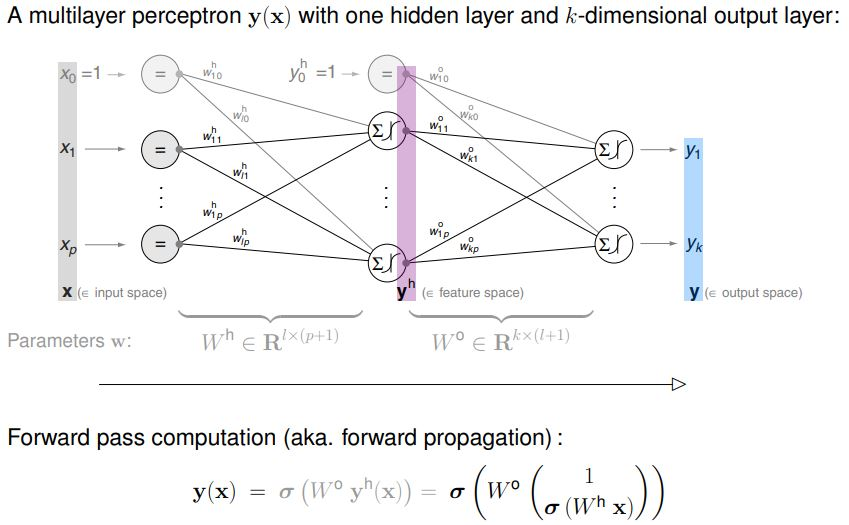
\includegraphics[width=0.8\textwidth]{MP}
\subsubsection{Forward propagation}
The input data is fed in the forward direction through the network. Each hidden layer accepts the input data, processes it as per the activation function and passes to the successive layer
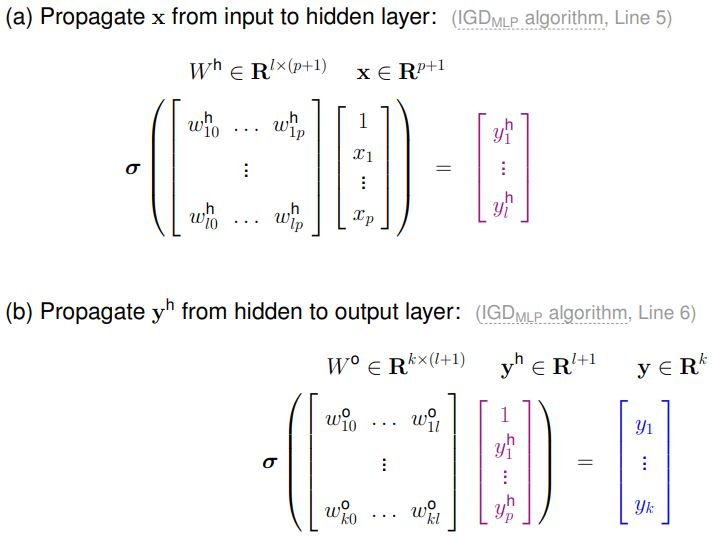
\includegraphics[width=0.8\textwidth]{forwardProp}
\textbf{Forward propagation: Batch Mode}
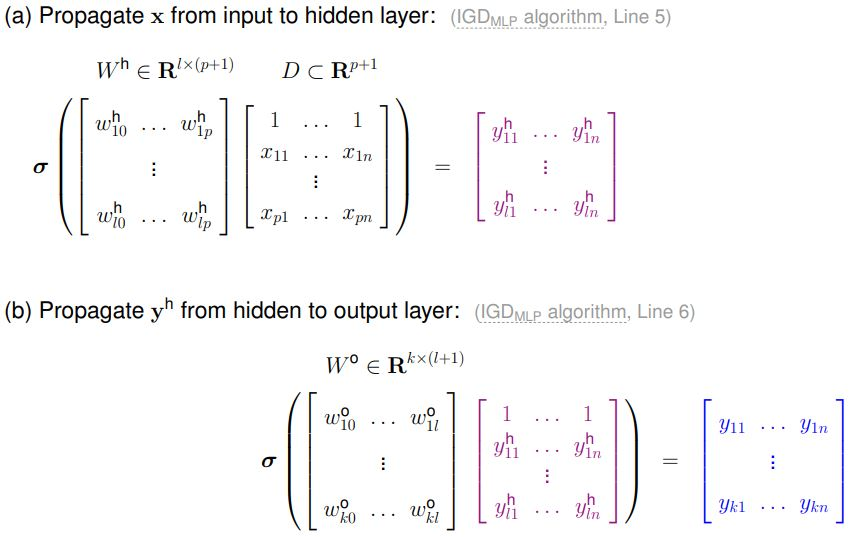
\includegraphics[width=0.8\textwidth]{forwardPropBatch}
\subsubsection{Backwards Propagation}
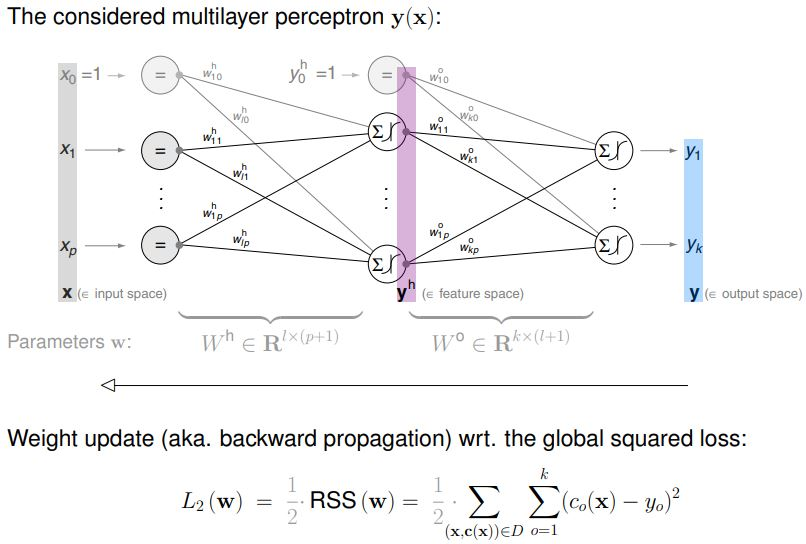
\includegraphics[width=0.8\textwidth]{BackwardProp}
\begin{itemize}
\item $L_2 (\textbf{w})$ usually contains various local minima
\end{itemize}
$$ \begin{bmatrix}
\dfrac{\delta L_2 (\textbf{w})}{\delta w^o_{10}} & \cdots & \dfrac{\delta L_2 (\textbf{w})}{\delta w^o_{1l}} \\
 & \vdots & \\
\dfrac{\delta L_2 (\textbf{w})}{\delta w^o_{k0}} & \cdots &  \dfrac{\delta L_2 (\textbf{w})}{\delta w^o_{kl}}
 \end{bmatrix} \equiv \nabla ^o L_2(\textbf{w}) $$

die selbe Formel gibt es nochmal nur mit "h" statt "o" \\
Update of weight matrix $W^o$: $W^o = W^o + \delta W^o $ mit: 
$$ \Delta W^o = - \eta \cdot \nabla ^o L_2(\textbf{w}) = \eta \cdot \displaystyle\sum_D  [(W^{oT} \delta ^o) \odot y^h (\textbf{x}) \odot (1 - y^h (\textbf{x}) )]_{1,...,l} \otimes \textbf{x} $$

weiß irgendwer was diese lange Formel sagen will? Nein? okay. 

\subsection{IGD for Multilayer Perceptrons}
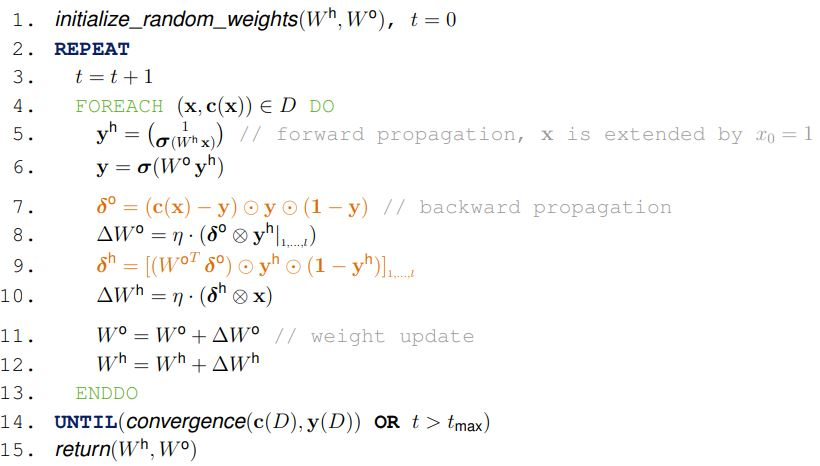
\includegraphics[width=0.8\textwidth]{MultiIGD}
\begin{itemize}
\item $\odot = $ \href{https://en.wikipedia.org/wiki/Hadamard_product_(matrices)}{Hadamard product}
\item $ \otimes  = \textbf{vw}^T $ \href{https://en.wikipedia.org/wiki/Dyadics}{dyadic product}
\end{itemize}
another formel for $ \nabla^o L_2 (\textbf{w})$: 

$$ \frac{\delta}{\delta w^o _ {ij}} = - \sum_D (c_i (\textbf{x}) - y_i(\textbf{x})) \cdot y_i(\textbf{x}) \cdot (1- y_i (\textbf{x})) \cdot y_j^h(\textbf{x}) $$ 

\section{Decision Trees}
\subsection{Splitting}

Das splitting von $X$ ist die Teilung in mutually exclusive Teilmengen $X_1, . . . , X_s$ alias $X = X_1 \cup ... \cup X_s$ mit $X_j \neq \emptyset$ and $X_j \cap X_j \neq \emptyset$, where $j, j' \in \{1, . . . , s\}, j \neq j'$.
Eine Teilung $X_1, ... , X_s$ von $X$ induces eine Teilung $D_1, . . . , D_s$ von $D$, bei der $D_j, j = 1, ... , s,$ als $\{(\textbf{x}, c(\textbf{x})) \in D | x \in X_j\}$ definiert wird. \\
Oder in Beispielen: Wir teilen unsere Pilze in 2 (oder mehr) Haufen anhand einer Eigenschaft, z.B. Farbe. Statt also einem Haufen beschrifteter Pilze (unser Beispieldatenset D) haben wir 3 Haufen: weiße Pilze, braune Pilze und rote Pilze. (die wiederum weiter aufgeteilt werden bis wir für jeden Haufen klar sagen können: essbar oder nicht essbar)\\

Die Teilung hängt von der Art der Eigenschaften/ Features ab. Diese können
\begin{itemize}
\item numerisch/ quantitative sein: Zahlen und Ratios, z.B. die Temperatur in °C, das Alter in Jahren oder Geld in Währung (Rechnen mit + \& - und/oder * \& / ergibt Sinn)
\item kategorisch/ Qualitative sein: Namen, Farben, IDs, Postleitzahlen, Hausnummern, etc. (nur Vergleichen [=, $\neq$ bzw. manchmal noch $<$ \& $>$] ergibt Sinn)
\end{itemize}

Daraus folgen verschiedene Teilmöglichkeiten:
\begin{itemize}
\item $m$-ary splitting induced by a (nominal) feature $A$ with finite domain (braune, weiße und rote Pilze):
$$A = \{a_1,...a_m\}: X = \{\textbf{x} \in X: \textbf{x}|_a = a_1 \} \cup ... \cup \{\textbf{x} \in X: \textbf{x}|_a = a_m \} $$
\item Binary splitting induced by a (nominal) feature A (Punkte vs keine Punkte):
$$ A' \subset A : X = \{\textbf{x} \in X: \textbf{x}|_a \in A' \} \cup \{\textbf{x} \in X: \textbf{x}|_a  \notin A' \} $$
\item Binary splitting induced by an ordinal feature A (Temp $<$25 °C und Temp $\geq $25°C): 
$$ v \in dom (A): X = \{\textbf{x} \in X: \textbf{x} |_a  \succeq v \} \cup \{\textbf{x} \in X: \textbf{x}|_a \prec  v \} $$
\item $\textbf{x}|a_i$ sind die \textbf{x} die eine eigenschaft $a_i$ erfüllen (z.B. braun)
\end{itemize}

\subsubsection{Possible criteria for splitting of X(t)}
\begin{enumerate}
\item \textbf{Size of D(t)}: $D(t)$ is not split if $|D(t)|$ is below a threshold.
\item \textbf{Purity of D(t)}: $D(t)$ is not split if all examples in $D(t)$ are members of the same class
\item \textbf{Impurity reduction of D(t)}: $D(t)$ is not split if its impurity reduction, $\Delta_\iota $, is below a threshold (wenn es sich nicht lohnt weil es sich nicht signifikant verbessert)
\end{enumerate}

\subsection{Decision Trees Definiton}

Let $X$ be a set of features and $C$ a set of classes. A decision tree $T$ for $X$ and $C$ is
a finite tree with a distinguished root node. A non-leaf node $t$ of $T$ has assigned
\begin{itemize}
\item[1] a set $X(t) \subset X$,
\item[2] a splitting of $X(t)$, and
\item[3] a one-to-one mapping of the
subsets of the splitting to its successors.
\end{itemize}
$X(t) = X$ iff $t$ is root node. A leaf node of $T$ has assigned a class from $C$.
\begin{itemize}
\item decision trees (DT) haben kein Problem mit Rauschen/ Labelnoise (falsch klassifizierte Beispiele) da wenn diese in der Minderheit sind nicht berücksichtigt werden (wenn ich 5 mal bei sonnigem, warmen, windstillen Wetter Sport mache und 1 mal nicht) haben wir ein geteilten Knoten (siehe Bild) und entscheiden und meistens für die Mehrheit (Sport machen). 
\item manchmal (essbar/ nicht essbar) ergibt jedoch auch eine andere Entscheidung Sinn
\item DT können nur klassifizieren nicht Regression 
\end{itemize}

\subsubsection{classification of some $\textbf{x} \in X$ given a decision tree T}
\begin{enumerate}
\item Find the root node $t$ of $T$
\item if $t$ is a non-leaf node, find among its successors that node $t'$ whose subset of
the splitting of $X(t)$ contains $\textbf{x}$. Repeat this step with $t = t'$
\item If $t$ is a leaf node, label $x$ with the respective class
\end{enumerate}

\textbf{The set of possible decision trees forms the hypothesis space $H$}
\begin{itemize}
\item The classification of an $x \in X$ determines a unique path from the root node of $T$ to some leaf
node of $T$
\item At each non-leaf node a particular feature of $x$ is evaluated in order to find the next node
along with a possible next feature to be analyzed
\end{itemize}
\subsubsection{Notations}
Let $T$ be a decision tree for $X$ and $C$, let $D$ be a set of examples [setting], and let $t$ be
a node of $T$. Then we agree on the following notation:
\begin{itemize}
\item  $X(t)$ denotes the subset of $X$ that is represented by $t$.
\item $D(t)$ denotes the subset of the example set $D$ that is represented by $t$, where
$D(t) = {(\textbf{x}, c(\textbf{x})) \in D | \textbf{x} \in X(t)}$. (see the splitting definition)
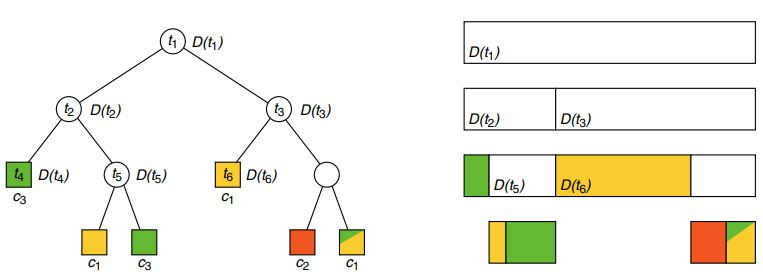
\includegraphics[width= \textwidth]{dTree}
\item The set $X(t)$ is comprised of those members $x$ of $X$ that are filtered by a path from the root
node of $T$ to the node $t$.
\item $leaves(T)$ denotes the set of all leaf nodes of $T$
\item ab hier: $t, T : X \rightarrow C$ statt $ y_t, y_T : X \rightarrow C$
\end{itemize}
\subsubsection{DT-construct}
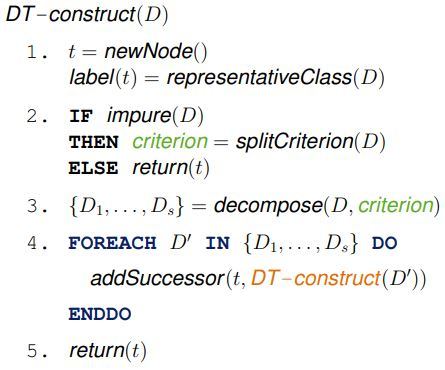
\includegraphics[width= \textwidth]{construct}
\begin{itemize}
\item Since $DT$-construct assigns to each node of a decision tree $T$ a class, each subtree of $T$ (as
well as each pruned version of a subtree of $T$) represents a valid decision tree on its own
\item $representativeClass(D)$ : Returns a representative class for the example set $D$. Note that, due to pruning, each node may become a leaf node.
\item $impure(D)$ Evaluates the (im)purity of a set $D$ of examples
\item $splitCriterion(D)$ Returns a split criterion for $X(t)$ based on the examples in $D(t)$.
\item $decompose(D, criterion)$ Returns a splitting of $D$ according to criterion
\item $addSuccessor(t, t')$ Inserts the successor $t'$ for node $t$
\end{itemize}
\subsubsection{DT-classify}
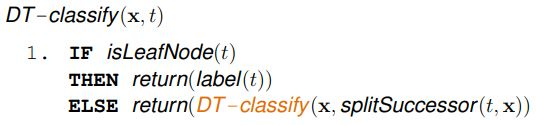
\includegraphics[width= \textwidth]{classify}
\begin{itemize}
\item $isLeafNode(t)$ Tests whether $t$ is a leaf node
\item $splitSuccessor(t, x)$ Returns the (unique) successor $t'$ of $t$ for which $x \in X(t')$ holds
\end{itemize}
\subsection{Evaluation of DT}
Um noch Bias zu haben (und somit für nicht gesehene Beispiele abstrahieren zu können) müssen wir den Baum jetzt noch kürzen. (Overfitting vermeiden)
\begin{enumerate}
\item Size: Among all decision trees of minimum classification error we choose the
one of smallest size
\item Classification Error: Quantifies the rigor according to which a class label is assigned to $x$ in a leaf node of $T$, based on the examples in $D$. If all leaf nodes of a decision tree $T$ represent a single example of $D$, the classification error of $T$ with respect to $D$ is zero. (Wollen wir meistens nicht)
\end{enumerate}
\subsubsection{measuring Size}
\begin{itemize}
\item Leaf node number (wie viele Endknoten)
\item Tree height (Längster Weg im Baum von Wurzel bis Blatt)
\item External path length (Summe aller Wege von Wurzel bis Blätter = der Platz den es braucht alle in einem Baum gespeicherten Regeln zu speichern)
\item Weighted external path length (wie external path lenght aber wir schauen für jeden Weg noch wie viele Beispiele aus $D$ klassifiziert werden) $\rightarrow $ Ein kurzer Weg der viel klassifiziert  + ein sehr langer weg der sehr wenig klassifiziert kann besser sein als 2 Halblange Wege (die beliebig aufteilend klassifizieren)
\item Weighted external path length ist meistens bevorzugt
\end{itemize}
\subsubsection{Classification Error}
$$ label(t) = \argmax_{c \in C} \dfrac{|(\textbf{x},c(\textbf{x}) \in D(t): c(\textbf{x}) = c)|}{|D(t)|} $$
\textbf{Missclassification rate}/ Error of node classifier t based on that:
$$ Err(t,D(t)) = \dfrac{|\{ \x , c( \x ) ) \in D (t) : c( \x ) \neq label(t) \} | }{|D(t)|} = 1 - \max_{c \in C} \dfrac{|\{ \x , c( \x ) ) \in D (t) : c( \x ) = c \} | }{|D(t)|} $$
\textbf{Misclassification rate} of decision tree classifier T: 
$$ Err(T,D) = \sum_{t \in leaves(T)} \frac{|D(t)|}{|D|} \cdot Err(t, D(t)) $$
argmax gibt das $\x $  zurück für das eine Funktion $f(\x )$ maximal ist, max gibt $ y (\x )$ zurück (Beispiel Wohnungspreise anhand der Lage: $argmax(\x ) =$  "Innenstadt" und $max(\x ) = $ "75000 Euro") (und genauso für argmin vs min) \\
\textbf{Misclassification cost} of node classifier t:
$$ Err_{cost}(t,D(t)) = min_{c' \in C} \sum_{c' \in C} \frac{|\{ (\x , c(\x )) \in D(t): c(\x )=c \}|}{|D(t)|} \cdot cost(c' | c) $$
\textbf{Misclassification costs} of decision tree classifier T:
$$ Err_{cost}(T,D) = \sum_{t \in leaves(T)} \frac{|D(t)|}{|D|} \cdot Err_{cost}(t, D(t)) $$
Wenn $c' = c$ ist $cost(c'|c)$ = 0, verschiedene c können verschiedene Kosten haben (es ist schlimmer einen toxischen Pilz als essbar einzustufen als einen essbaren als toxisch)

\subsection{Impurity Functions}
An impurity function $\iota : [0;1]^k \rightarrow R$ (mit $k \in N $) is a function defined on the standard
$k-1- simplex$, denoted $\Delta ^{k-1} $, for which the following properties hold:
\begin{enumerate}
\item $\iota $ becomes minimum at points (1,0,...,0), (0,1,...,0),..., (0,...,0,1)
\item $\iota $ is symmetric with regard to its arguments, $p_1, ... , p_k $
\item $\iota $ becomes maximum at point $(1/k, ..., 1/k)$
\end{enumerate}
simplex = einfachste Form zwischen Punkten in k- Dim raum (also k = 3 $\rightarrow$ Dreieck)? \\

\subsubsection{Strict Impurity Function} 
genauso wie Impurity aber 
\begin{itemize}
\item[3.] wird zu:  $ \iota(\lambda p + (1 - \lambda ) p' ) > \lambda \iota (p) + ( 1 - \lambda ) \iota (p'), 0 < \lambda < 1, p \neq p'  $
\end{itemize}

Wenn $\iota $ eine stricte impurity funktion ist gilt:

$$ \Delta \iota ( D, \{D_1, ..., D_s\} ) \geq 0 $$

\subsubsection{Impurity of an Example Set}
Impurity of $D = \iota(D) $ :

$$ \iota (D) = \iota (\frac{|\{ (\x , c( \x ) ) \in D: c(\x ) = c_1 \}|}{|D|}, ... , \frac{|\{ (\x , c( \x ) ) \in D: c(\x ) = c_k \}|}{|D|} ) $$

eine Funktion ist maximal impure wenn alle ihr zugeordneten Klassen c gleich wahrscheinlich sind (50\% Wahrscheinlichkeit essbar, 50\% Wahrscheinlichkeit toxisch). 
\subsubsection{Impurity Reduction}
D aufgeteilt in $D_1, ..., D_s$, durch das splitting von X, dann ist die resulting impurity reduction: 

$$ \Delta \iota (D, \{D_1,..., D_s\}) = \iota (D) - \sum_{j=1}^s \frac{|D-j|}{|D|} \cdot \iota (D_j) $$

\subsubsection{Impurity Functions Based on the misclassification Rate}
Definition für 2 classes:
$$ \iota_{misclass} (p_1,p_2) = 1 - max \{p_1,p_2\} = 
\begin{cases}
p_1      & \quad \text{if } 0 \leq p_1 \leq 0.5 \\
1-p_1  & \quad \text{otherwise}
\end{cases} $$
$$ \iota_{misclass} (D) = 1 - max \{ \frac{|\{ (\x , c(\x )) \in D: c(\x ) = c_1 \}|}{|D|}, \frac{|\{ (\x , c(\x )) \in D: c(\x ) = c_2 \}|}{|D|}\} $$
Definition für k classes: 
$$ \iota_{misclass} (p_1, ... , p_k) = 1 - \max_{i = 1, ..., k} p_i $$

$$ \iota_{misclass} (D) = 1 - \max_{c \in C}  \frac{|\{ (\x , c(\x )) \in D: c(\x ) = c \}|}{|D|} $$
Er hat in dem Video erklärt warum er hier plötzlich $p_1$ und $p_2$ benutzt statt $c_1$ und $c_2$, hat allerdings nicht so viel Sinn ergeben. 
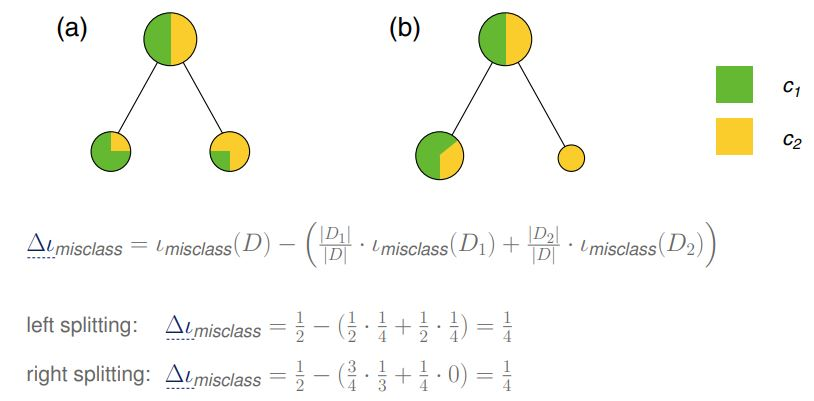
\includegraphics[width = \textwidth]{impurity}
Das Bild erklärt das Rechnen besser als alle Formeln.

\subsection{Entropy}

Let $A$ denote an event and let $P(A)$ denote the occurrence probability of $A$. Then the entropy (self-information, information content) of $A$ is defined as $ - \log _2 (P(A)) $. Let $A$ be an experiment with the exclusive outcomes (events) $A_1, . . . , A_k$. Then the mean information content of $A$, denoted as $H(A)$, is called Shannon entropy or entropy of experiment $A$ and is defined as follows:

$$ H(A) = - \sum_{i=1}^{k} P(A_i) \cdot \log _2 (P(A_i)) $$

The smaller the occurrence probability of an event, the larger is its entropy. An event that is
certain has zero entropy

\subsubsection{Conditional Entropy}

Let $\mathcal{A}$ be an experiment with the exclusive outcomes (events) $A_1, ... , A_k$, and let $\mathcal{B}$ be another experiment with the outcomes $B_1, ... , B_s$. Then the conditional entropy
of the combined experiment $ (\mathcal{A} | \mathcal{B} )$ is defined as follows:

$$ H(\mathcal{A} | \mathcal{B} ) = \sum_{j = 1}^s P(B_j)\cdot H(\mathcal{A} | \mathcal{B} _j ) $$

mit: $ H(\mathcal{A} | \mathcal{B} _j ) = - \sum_{i = 1}^k P(A_i | B_j )\cdot \log _2 (P (A_i | B_j ))$

\subsubsection{Information Gain} 

$$  H(\mathcal{A}) - H(\mathcal{A} | \mathcal{B} ) = H(\mathcal{A}) - \sum_{j = 1}^s P(B_j)\cdot H(\mathcal{A} | \mathcal{B} _j ) $$

\begin{itemize}
\item Information gain is defined as reduction in entropy
\item In the context of decision trees, experiment $\mathcal{A}$ corresponds to classifying feature vector \textbf{x} with regard to the target concept. A possible question, whose answer will inform us about which
event $A_i \in \mathcal{A}$ occurred, is the following: “Does \textbf{x} belong to class $c_i$?”
Likewise, experiment $\mathcal{B}$ corresponds to evaluating feature B of feature vector \textbf{x}. A possible question, whose answer will inform us about which event $B_i \in \mathcal{B} $ occurred, is the following: “Does \textbf{x} have value $b_j$ for feature $B$?”
\item Since $H(\mathcal{A})$ is constant, the feature that provides the maximum information gain (= the
maximally informative feature) is given by the minimization of $H(\mathcal{A} | \mathcal{B} )$.
\end{itemize}

\subsubsection{Impurity Functions Based on Entropy}
Tippen braucht zu viel Zeit, die Klausur ist morgen, also Screenshots for now:

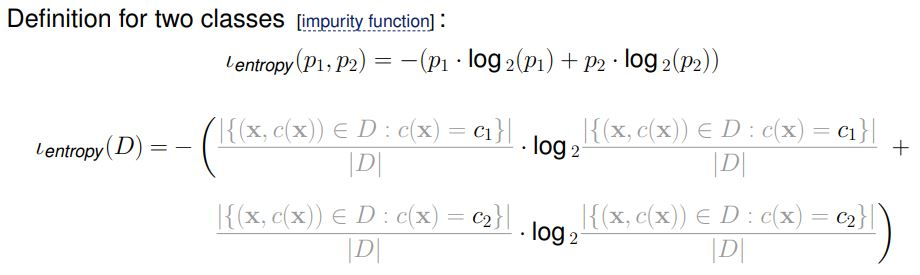
\includegraphics[width = \textwidth]{impureEntropy2}
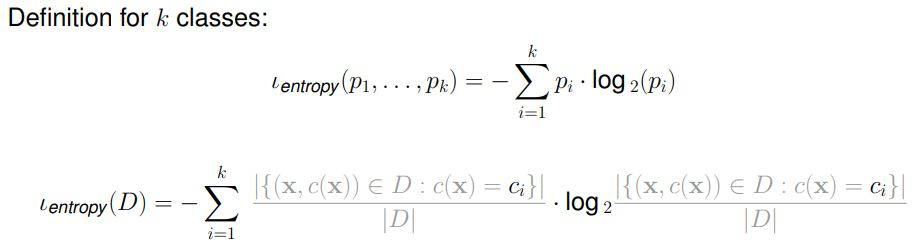
\includegraphics[width = \textwidth]{impureEntropyk}
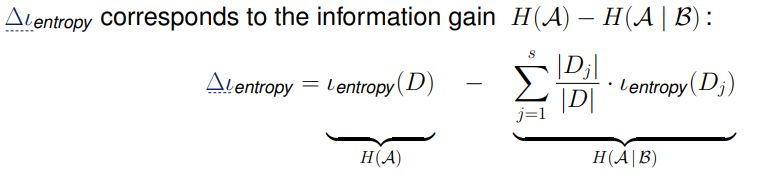
\includegraphics[width = \textwidth]{lentropy}
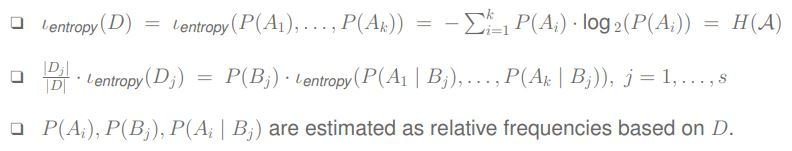
\includegraphics[width = \textwidth]{lentropy2}

\subsubsection{Impurity Functions Based on the Gini Index}
Wurde in der VL nicht besprochen (ist aber in den Folien) ich lass es mal weg. Man findet es \href{ https://webis.de/downloads/lecturenotes/machine-learning/unit-en-decision-trees-impurity.pdf }{hier (ich bin ein Link)} ab Folie 33.

\subsection{Decision Tree Algorithms}
\subsubsection{ID3 Algorithm}
Characteristics of the ID3 algorithm:
\begin{enumerate}
\item Each splitting is based on one nominal feature and considers its complete
domain. Splitting für Feature A: $A = \{a_1,...a_m\}: X = \{\textbf{x} \in X: \textbf{x}|_a = a_1 \} \cup ... \cup \{\textbf{x} \in X: \textbf{x}|_a = a_m \} $
\item Splitting criterion is information gain.
\end{enumerate}
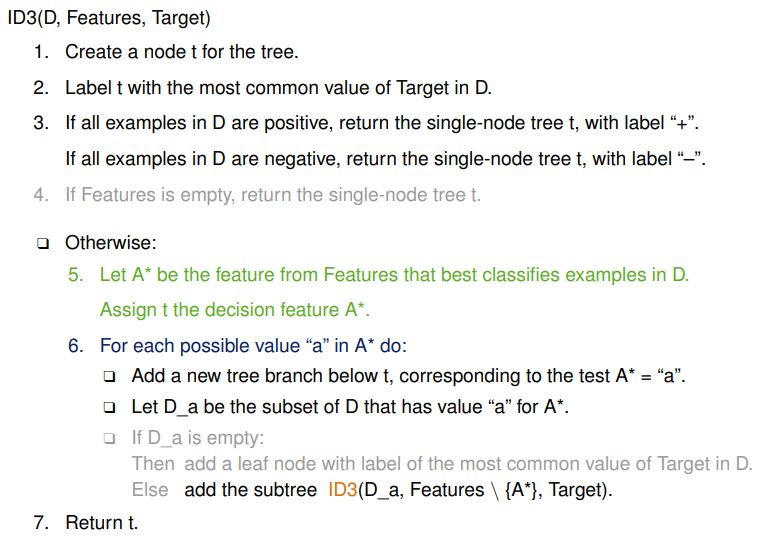
\includegraphics[width = \textwidth]{ID3Text}
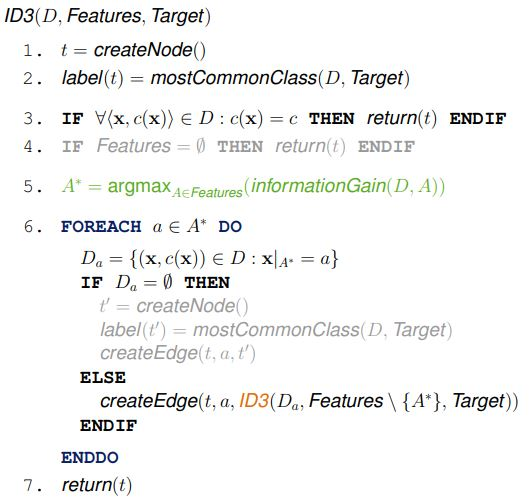
\includegraphics[width = \textwidth]{ID3}
\begin{itemize}
\item Step 3 of of the ID3 algorithm checks the purity of D and, given this case, assigns the unique
class c, ($c \in  dom(Target)$), as label to the respective node.
\item The smaller $H(C | feature)$ is, the larger becomes the information gain. Hence, the difference
$H(C) - H(C | feature)$ needs not to be computed since $H(C)$ is constant within each recursion step.
\end{itemize}

\subsubsection{ID3 Beispiel}
\includegraphics[width = \textwidth]{Pilze}
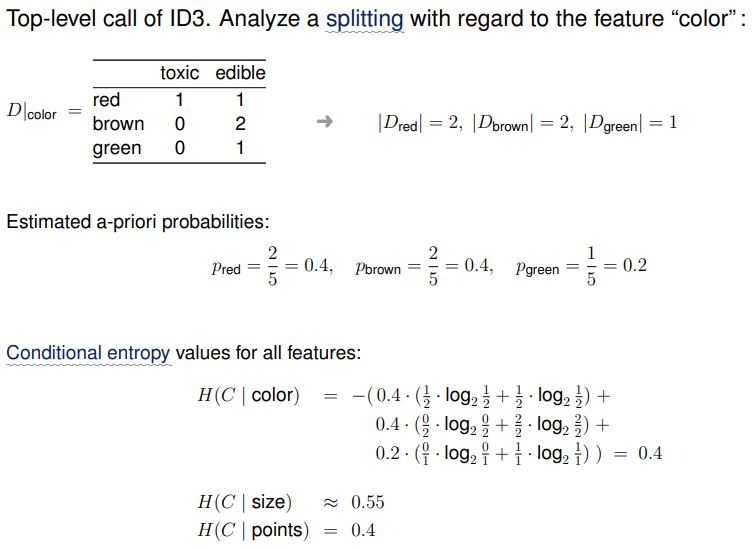
\includegraphics[width = \textwidth]{ID3Pilze}
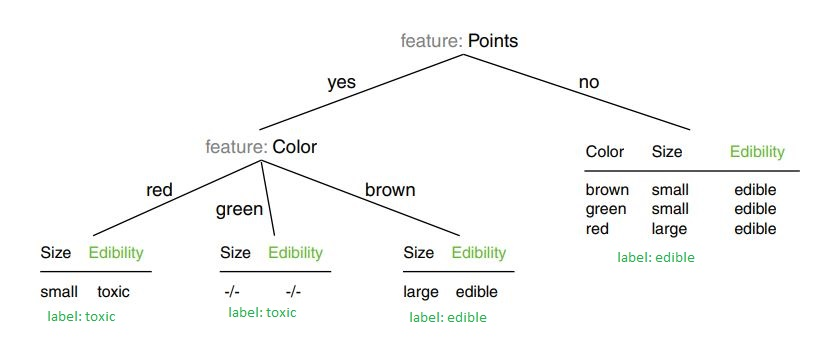
\includegraphics[width = \textwidth]{ID3Baum}

\subsubsection{ID3 Inductive Bias}
Inductive bias is the rigidity in applying the (little bit of) knowledge learned from a
training set for the classification of unseen feature vectors.
Observations:
\begin{itemize}
\item Decision tree search happens in the space of all hypotheses. $\rightarrow$ The target concept is a member of the hypothesis space.
\item To generate a decision tree, the ID3 algorithm needs per branch at most as
many decisions as features are given. $\rightarrow$ no backtracking takes place and the decision tree is a result of local optimization
\end{itemize}
 
Where the inductive bias of the ID3 algorithm becomes manifest:
\begin{itemize}
\item Small decision trees are preferred
\item Highly discriminative features tend to be closer to the root.
\end{itemize}
\begin{center}
\textit{Is this justified?}
\end{center}
\subsubsection{CART Algorithm}
Characteristics of the CART algorithm: Each splitting is binary and considers one feature at a time and  Splitting criterion is the information gain or the Gini index. 
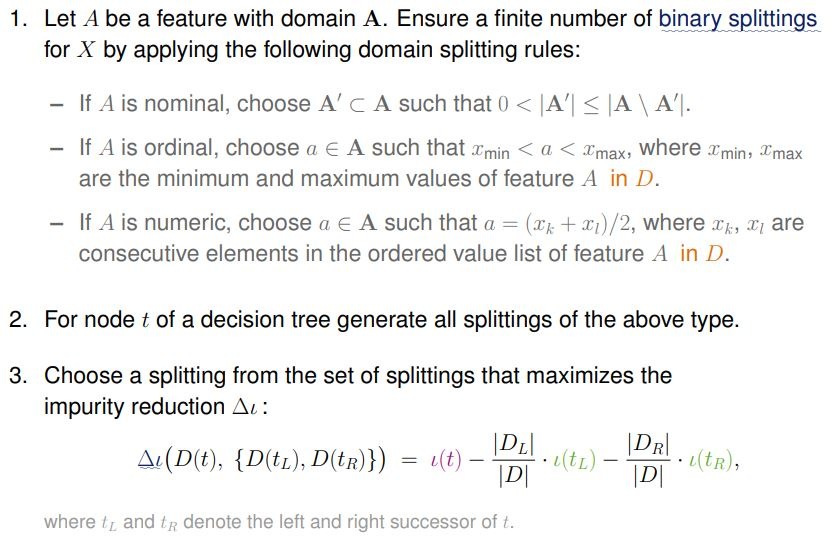
\includegraphics[width = \textwidth]{cart}
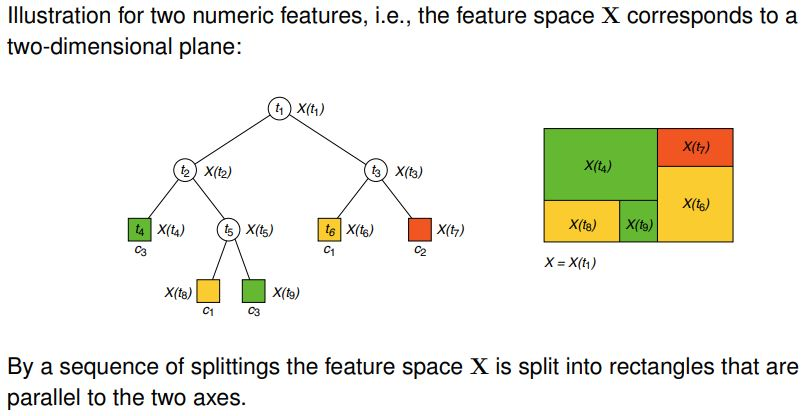
\includegraphics[width = \textwidth]{cartTree}
\subsection{Decision Tree Pruning}

\end{flushleft}
\end{document}
